\section{Quantum Dense Coding}
Il Quantum Dense Coding (o Superdense Coding) è una tecnica che permette di mappare diversi bit classici su un certo numero di Qubit. In particolare, per il superdese coding, si cerca di mappare 2 bit classici su di una singola coppia EPR condivisa tra trasmettitore e ricevitore. Quindi, quello che il trasmettitore cerca di fare è mappare la coppia di bit andando ad agire sul qubit in suo possesso, per poi inviarlo al trasmettiore, che con entrambii qubit, decirerà l'informazione. La pecca principale del superdense coding è dovuta all'ipotesi di canale perfetto, quindi un canale che non prevede errori ne di tipo bit flip ne di tipo phase flip. 

Supponiamo che inizialmente, quindi, Alice e Bob abbiano condiviso una coppia EPR tra i due. Di tale coppia, Alice ha un Qubit e Bob ne ha un altro. Alice decide se eseguire o meno le seguenti operazioni sul suo Qubit, in base a quale coppia di bit voglia inviare. Le regole che si vanno a seguire sono le seuenti:
\begin{itemize}
    \item Nel caso Alice voglia trasmettere \textbf{00}: Allora non va ad effettuare alcuna operazione sul suo qubit
    \item Nel caso Alice voglia trasmettere \textbf{01}: Allora va ad applicare una porta \(X\) sul suo Qubit
    \item Nel caso Alice voglia trasmettere \textbf{10}: Allora va ad applicare una porta \(Z\) sul suo Qubit
    \item Nel caso Alice voglia trasmettere \textbf{11}: Allora va ad applicare una porta \(iY\), che è la combinazione di \(X\) e \(Z\). Più precisamente: \(iY = Z X\).
\end{itemize}

Quindi è possibile definire un circuito per il superdense coding visualizzabile alla figura [\ref{img:superdense-coding}]. Tale immagine è stata presa da \cite{superdense_img}:

\begin{figure}[H]
\centering
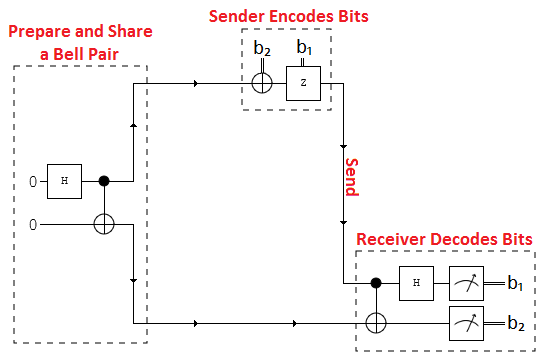
\includegraphics[width=.7\textwidth]{fig/Chapter-2/chapter-3/superdense-coding.png}
\caption{Superdense Coding circuito concettuale}\label{img:superdense-coding}
\end{figure}

\subsubsection{Matematica del superdense coding}
Per capire al meglio cosa succede, andiamo per ordine, partiamo dalla coppia EPR condivisa tra Alice e Bob (si consiglia di guardare l'immagine [\ref{img:superdense-coding}] mano a mano che si va avanti con i calcoli):
\[
\ket{\Phi^+} = \frac{1}{\sqrt{2}}(\ket{0_a}\ket{0_b} + \ket{1_a \_b})
\]

Immaginiamo di voler trasmettere la coppia di bit \(11\). Tale coppia, seguendo le regole predecedenti, va ad attivare sia la porta \(X\) e sia la porta \(Z\), per ottenere la porta \(iY\). Tale porta è definita come:
\[
iY =
\begin{bmatrix}
0 & 1 \\
-1 & 0
\end{bmatrix}
\Longleftrightarrow
\begin{cases}
\ket{0} \rightarrow - \ket{1} \\
\ket{1} \rightarrow \ket{0}
\end{cases}
\]

Andando a considerare l'applicazione di tale porta sul Qubit di alice si otterrebbe:
\[
\ket{\psi} = \frac{1}{\sqrt{2}}(-\ket{1_a} \ket{0_b} + \ket{0_a}\ket{1_b})
\]

Una volta effettuate le due operazioni, Alice invia il Qubit a Bob, Bob avrà quindi una coppia che sarà:
\[
\ket{\psi} = \frac{1}{\sqrt{2}} (-\ket{10}+\ket{01})
\]

Bob, da parte sua, applica una C-Not tra i due, considerando come controllore il Qubit ricevuto da Alice, ottenendo:
\[
\ket{\psi} = \frac{1}{\sqrt{2}} (-\ket{11} + \ket{01})
\]
Che portà anche essere visto come:
\[
\ket{\psi}= \frac{1}{\sqrt{2}} (\ket{0} - \ket{1}) \otimes \ket{1}
\]

Bob applica la porta di Hadamard sul Qubit di Alice, ottenendo:
\[
\ket{\psi} = \frac{1}{\sqrt{2}}(\ket{+} - \ket{-}) \otimes \ket{1}
\]

Ma ricordando che: \(\ket{1} = \frac{1}{\sqrt{2}}(\ket{+} - \ket{-})\), allora si ottiene:
\[
\ket{\psi} = \ket{1} \otimes \ket{1} = \ket{11}
\]

Che, misurato sulla base canonica, darà con probabilità del \(100 \%\) il risultato \(11\). 

Questo ragionamento sarebbe applicabile anche per le altre coppie.